\documentclass[letterpaper, 10 pt, conference]{ieeeconf}  % Comment this line out
                                                          % if you need a4paper
%\documentclass[a4paper, 10pt, conference]{ieeeconf}      % Use this line for a4
                                                          % paper

\IEEEoverridecommandlockouts                              % This command is only
                                                          % needed if you want to
                                                          % use the \thanks command
\overrideIEEEmargins
% See the \addtolength command later in the file to balance the column lengths
% on the last page of the document

% This is needed to prevent the style file preventing citations from linking to 
% the bibliography
\makeatletter
\let\NAT@parse\undefined
\makeatother

\usepackage[dvipsnames]{xcolor}

\newcommand*\linkcolours{ForestGreen}
\usepackage{times}
\usepackage{graphicx}
\usepackage{amssymb}
\usepackage{gensymb}
\usepackage{amsmath}
\usepackage{bbm}
\usepackage{breakurl}
\def\UrlBreaks{\do\/\do-}
\usepackage{url,hyperref}
\hypersetup{
colorlinks,
linkcolor=\linkcolours,
citecolor=\linkcolours,
filecolor=\linkcolours,
urlcolor=\linkcolours}

\usepackage{algorithm}
\usepackage{algorithmic}

\usepackage[labelfont={bf},font=small]{caption}
\usepackage[none]{hyphenat}

\usepackage{mathtools, cuted}

\usepackage[noadjust, nobreak]{cite}
\def\citepunct{,\,} % Style file defaults to listing references separately

\usepackage{tabularx}
\usepackage{amsmath}
\usepackage{bm}

\usepackage{float}

\usepackage{pifont}% http://ctan.org/pkg/pifont
\newcommand{\cmark}{\ding{51}}%
\newcommand{\xmark}{\ding{55}}%

\newcommand*\diff{\mathop{}\!\mathrm{d}}
\newcommand*\Diff[1]{\mathop{}\!\mathrm{d^#1}}
\newcommand*\imgres{600}

\newcolumntype{Y}{>{\centering\arraybackslash}X}

\usepackage[]{placeins}


\newcommand\extraspace{3pt}

\usepackage{placeins}

\usepackage{tikz}
\newcommand*\circled[1]{\tikz[baseline=(char.base)]{
            \node[shape=circle,draw,inner sep=0.8pt] (char) {#1};}}

\usepackage[framemethod=tikz]{mdframed}

\usepackage{afterpage}

\usepackage{stfloats}

\usepackage{atbegshi}
\newcommand{\handlethispage}{}
\newcommand{\discardpagesfromhere}{\let\handlethispage\AtBeginShipoutDiscard}
\newcommand{\keeppagesfromhere}{\let\handlethispage\relax}

% New commands added by stephen
\newcommand{\norm}[1]{\left\lVert#1\right\rVert}

\AtBeginShipout{\handlethispage}

\usepackage{comment}

% The following packages can be found on http:\\www.ctan.org
%\usepackage{graphics} % for pdf, bitmapped graphics files
%\usepackage{epsfig} % for postscript graphics files
%\usepackage{mathptmx} % assumes new font selection scheme installed
%\usepackage{times} % assumes new font selection scheme installed
%\usepackage{amsmath} % assumes amsmath package installed
%\usepackage{amssymb}  % assumes amsmath package installed

\title{\LARGE \bf
Model Discovery on Population and Video Datasets
}

\author{Stephen Jonany$^{1}$ % <-this % stops a space
\thanks{$^{1}$Stephen is a Master's student in Applied Mathematics at the 
University of Washington.
Email: sjonany@uw.edu.}%
}

\begin{document}


\maketitle
\thispagestyle{plain}
\pagestyle{plain}


%%%%%%%%%%%%%%%%%%%%%%%%%%%%%%%%%%%%%%%%%%%%%%%%%%%%%%%%%%%%%%%%%%%%%%%%%%%%%%%%
\begin{abstract}
We apply model discovery techniques such as dynamic mode decomposition (DMD), time-delay embedding and Sparse Identification of Nonlinear Dynamics (SINDy) to summarize the dynamics encoded within the provided population and video datasets. We also compare the efficacy of these different approaches with various performance metrics such as KL divergence, AIC and BIC.

\end{abstract}

%%%%%%%%%%%%%%%%%%%%%%%%%%%%%%%%%%%%%%%%%%%%%%%%%%%%%%%%%%%%%%%%%%%%%%%%%%%%%%%%
\section{Introduction and Overview}
Many interesting real-world phenomena, such as population growth, can be represented as values that fluctuate over time. The problem of predicting future values given a limited historical sample is thus a very a salient problem to solve. Many model discovery approaches attempt to predict the summarized dynamics behind given historical samples, before using these simplified dynamics to extrapolate future time points.

Among the various model discovery approaches, we will consider dynamic mode decomposition (DMD)\cite{schmid2010dmd}, time-delay embedding and Sparse Identification of Nonlinear Dynamics (SINDy)\cite{brunton2016sindy}. By using evaluation metrics such as KL divergence, AIC and BIC, these models will then be evaluated not only based on how well they fit the provided data, but also on their simplicity.

We will work with two datasets to test these approaches. The first dataset contains yearly hare and lynx populations. The second dataset is a video snippet of a Belousov-Zhabotinsky chemical oscillator movie.

%%%%%%%%%%%%%%%%%%%%%%%%%%%%%%%%%%%%%%%%%%%%%%%%%%%%%%%%%%%%%%%%%%%%%%%%%%%%%%%%
\section{Theoretical Background}
\subsection{Singular Value Decomposition}
\label{section:svd}
Singular value decomposition (SVD) is a dimensionality reduction technique that aims to decompose a matrix $M$ into the product of three matrices $U\Sigma V^*$. The implementation that we are using is the economy SVD, where if $M$, the original matrix, is of dimension $m \times n$ and we have chosen a low rank $r \le min(m,n)$, then both $U$ and $V$ are composed of orthonormal column vectors, with $U$ of dimension $m \times r$, and $V$ of dimension $n \times r$. $\Sigma$ is a square diagonal matrix of dimension $r \times r$, and the diagonal values are often referred to as the singular values.

The singular values can be thought of as a measure of the importance of the corresponding column vectors of $U$ and $V$ in reconstructing the original matrix $M$. By selecting the top $r$ values of $\Sigma$ and the corresponding $r$ columns of $U$ and $V$, one can reconstruct an approximation of the matrix $M$. One useful metric for deciding on how many top singular values to keep is the total energy, as defined in Equation \ref{eq:energy}.

\begin{equation}
Energy(r) = \frac{\sum_{i=1}^r \sigma_i^2}{ \sum_{i=1}^n \sigma_i^2}
\label{eq:energy}
\end{equation}
The energy metric measures how much of the original variance of the data is retained if we only keep the top $U$  and  $V$  components corresponding to the top $r$ singular values.

There are also some intuitive interpretations of $U$ and $V$. The columns of $U$ serve as the basis vectors of the column space of $M$. Likewise, the columns of $V$ serve as the basis vectors of the row space of $M$. Thus, if $M$ is composed of multiple time series, where each row is a single entity changing over time, say, the hare population across the years, then we can say that the hare population time series can be well approximated by a linear combination of the columns of $V$.

\subsection{Dynamic Mode Decomposition (DMD)}
\label{section:dmd}
DMD\cite{schmid2010dmd} is a model discovery technique for time-series prediction. There are two major assumptions of DMD, the first being that future states can be represented as a linear combination of historical states, the second being that the linear transformation that moves the states forward in time can be well-approximated in a lower dimension.

We first discuss the assumption that there is a linear relationship between the past and the future. Consider state vector $\bm{x_i}$, which represents an $n$-dimensional observation in a specific time $t_i$. We assume that we have $m$ such observations from $\bm{x_1}$ to $\bm{x_m}$, where the time increment between each observation is kept constant. Let $X$ be the collection of observations from times $1$ to $m$ stacked as column vectors, and $X'$ be similarly defined, except that it corresponds to observations from times $2$ to $m+1$. Then, DMD assumes there is a linear transformation $A$ from $X$ to $X'$ as seen in Equation \ref{eq:dmd_assumption}.

\begin{equation}
AX = X'
\label{eq:dmd_assumption}
\end{equation}
Note that the dimension of X and X' are $n \times m$, because there are $m$ column vectors, each of length $n$. This means $A$ is of the dimension $n \times n$.

We now discuss the second component of DMD: a low-rank approximation of the $A$ matrix. Although Equation \ref{eq:dmd_assumption} can be solved as a normal regression problem, in practice, one tackles a lower-dimensional version for computational tractability. The steps are as follows.

%% Begin DMD steps
\begin{enumerate}
\item{\textbf{SVD on X}.
We pick a low rank $r$ following Section $\ref{section:svd}$, and obtain a low-rank approximation of $X$ like so, 
\begin{equation}
X \approx \Tilde{U} \Tilde{\Sigma}\Tilde{V^*}
\end{equation}
where $\Tilde{U}$ is $n \times r$, $\Tilde{\Sigma}$ is $r \times r$ and $\Tilde{V}$ is $m \times r$.
}

\item{\textbf{Reduce the dimension of $A$}.
In this step, we reduce the dimension of $A$ from $n \times n$ to $r \times r$. We achieve this by performing a similarity transform of $A$ onto the columns of $U$. Since $AX = X'$, then $A = X' X^{\dagger} \approx X' ( \Tilde{U} \Tilde{\Sigma}\Tilde{V^*})^\dagger =  X' \Tilde{V} \Tilde{\Sigma}^{-1}\Tilde{U}^*$. We then use this to obtain the similarity transformed, lower-rank $\Tilde{A}$ as follows.
\begin{equation}
\Tilde{A} = \Tilde{U}^*A \Tilde{U} = \Tilde{U}^*X' \Tilde{V} \Tilde{\Sigma}^{-1}
\end{equation}
A useful property is that the similarity transformation preserves the nonzero eigenvalues of $A$. Thus, we can avoid working with the high-dimensional $A$ and instead focus on the lower-dimensional $\Tilde{A}$.
}

\item{}\textbf{Eigendecomposition of $\Tilde{A}$}.
Through eigendecomposition, we achieve the following:
\begin{equation}
    \Tilde{A}W = W\Lambda
\end{equation}
where the columns of $W$ are the eigenvectors of $\Tilde{A}$, and the $\Lambda$ is a diagonal matrix consisting of the eigenvalues of $\Tilde{A}$, which are also the eigenvalues of the original $A$. Thus, $\Lambda$ contains the DMD eigenvalues themselves.

\item{\textbf{DMD mode $\Phi$}. We have the eigenvalues, and now we will find the DMD modes. Tu et al. \cite{tu2013dmd} calculates the high-dimensional DMD modes like so.
}
\begin{equation}
    \Phi = X' \Tilde{V} \Tilde{\Sigma}^{-1} W
\end{equation}
\end{enumerate}
%% End DMD Steps

Now that we have the DMD mode $\Phi$, of dimension $n \times r$, and the diagonal matrix containing the eigenvalues, $\Lambda$, of dimension $r \times r$, the we can obtain the low-rank projection of the initial condition $\bm{x_1}$, referred to as $\bm{b}$, like so.

\begin{equation}
    \bm{b} =  \Phi^{\dagger} \bm{x_1}
\label{eq:dmd_predict}
\end{equation}

Finally, we are able to predict future states $x_k$ like so.
\begin{equation}
    \bm{x_k} =  \Phi \Lambda ^{k-1}\bm{b}
\end{equation}

Equation \ref{eq:dmd_predict} is reminiscent of exponentiating an eigendecomposed matrix, where one simply has to exponentiate the eigenvalue matrix, and leave the eigenvector matrix untouched. In this case, we are applying an approximation of $A$, the matrix that supposedly carries our state vectors forward in time, $k-1$ times, hence bringing $\bm{x_1}$ to a predicted value of $\bm{x_k}$. Furthermore, we have done so through low-rank approximations, allowing us not to deal with the high-dimensional $A$ matrix.

In summary, DMD enables us to summarize the dynamics that move state variables forward in time in a given set of time series data, and allows us to predict future states.

\subsection{Time-delay Embedding}
\label{section:time_delay}
A major assumption of DMD is that Equation \ref{eq:dmd_assumption} mostly holds true. That is, we assume that the future states can be expressed as a linear combination of the historical states. For cases where this assumption is majorly violated, a solution would be to project the state variables into a different functional space. One such projection approach is time-delay embedding.

In time-delay embedding, we increase the state space dimension by $k$-fold, where $k$ indicates how many future state variables one wants to include in every column of the transformed matrix. If one starts with an original matrix $M$ of dimension $n \times m$, where each $n$-dimensional column vector is a measurement in time, then with $k$ embedding, the higher dimensional matrix $M'$ is of dimension $nk \times (m-k+1)$. The first column will then contain $x_1, ..., x_k$ stacked up row-by-row, and the second column will contain $x_2, ..., x_{k+1}$, going to the last column, which contains $x_{m-k+1},..., x_{m}$.

As we will see later on, time-delay embedding could help improve the efficacy of the DMD approach.

\subsection{Sparse Identification of Nonlinear Dynamical Systems (SINDy)}
\label{section:sindy}
SINDy \cite{brunton2016sindy} is a model discovery approach that one can use to model systems believed to be produced by ordinary different equations (ODEs). The problem setup that is relevant for our given datasets is such that we are provided with observations of state variables $\bm{x(t_1)}, ... , \bm{x(t_m)}$, corresponding to measurements taken at regular intervals in time, each state variable is of dimension $n$ . Our goal is to find the first order ODE $\frac{d\bm{x}}{dt} = f(\bm{x}) = f(x_1, x_2, ..., x_n)$.

We make a simplifying assumption that the true ODE is well approximated by a linear combination of a library of functions of the state vector. That is, we assume that we have already chosen a list of $L$ functions $f_1(\bm{x}), f_2(\bm{x}), ... ,f_L(\bm{x})$. Let us focus on just the recovery of the ODE for the first out of the $n$ state variables, $x_1$. The ODE can be expressed like so:

\begin{equation}
\frac{dx_1}{dt} = \sum_{i=1}^{L} c_i f_i(x_1, x_2, ..., x_n) 
\label{eq:sindy_library}
\end{equation}
where $c_i$'s, the weights applied to the library functions, are what we wish to discover.

Given this assumption, and given the data matrix $X$ of dimension $n \times m$, composed of $\bm{x(t_1)}, ... , \bm{x(t_m)}$ arranged along the column vectors, and we can obtain the $c_i$'s with the following steps.

\begin{enumerate}

\item{\textbf{Obtain $\frac{dx_1}{dt}$ labels,} $\bm{b}$.}
From the provided matrix $X$, we would like to obtain the values of $\frac{dx_1(t)}{dt}$ for $t_2, t_3, ..., t_{m-1}$. We approximate these values using centered finite difference like so:
\begin{equation}
\frac{dx_1(t_i)}{dt} \approx \frac{x_1(t_{i+1}) - x_1(t_{i-1})}{2d}
\end{equation}
, where $d$ is the time increment between each time snapshot. Note that we throw out $t_1$ and $t_m$, and so are left with $m-2$ labels.
Let this $(m-2) \times 1$ column vector be $\bm{b}$.

\item{\textbf{Create the function library matrix} $A$}.
We next generate the matrix $A$, of dimension $(m-2) \times L$, where each column $i$ of this matrix is taking the one out of the $L$ functions, $f_i$, and applying it to each of the $m-2$ column in $X$ (without the first and last time point), a measurement in a single time. That is, $A_{ij} = f_j(\bm{x(t_{i+1})})$.

\item{\textbf{Solve for function weights}, \textbf{c}}.
The formulation provided in Equation \ref{eq:sindy_library} means that to find the weight vector $\bm{c}$, of dimension $L \times 1$, we just have to solve the familiar problem $A\bm{c} = \bm{b}$. We will use a sparse regression method, Lasso\cite{tibshirani1994lasso}, to find the best $\bm{c}$ that balances data fit and overfitting. This will allow us to subselect only a few of the library functions, keeping our final predicted ODEs more compact. For a more thorough discussion on Lasso, please refer to the previous writeup on the MNIST dataset.
\end{enumerate}

We have discussed how to find the best set of function library weights to describe $\frac{dx_1}{dt}$. One would then repeat the above steps $n-1$ more times to obtain the ODEs for the other state variables. All in all, one would end up with $L \times n$ coefficients to describe all $n$ ODEs.

With the ODEs in hand, one can employ various ODE solvers such Runge–Kutta methods in order to predict any future state $\bm{x(t)}$. 

\subsection{Lotka-Volterra}
\label{section:lotka_volterra}
Lotka-Volterra equations model the populations of predator and prey with a set of ODEs like so.
\begin{equation}
\begin{split}
\frac{dx}{dt} = (b - py) x \\
\frac{dy}{dt} = (rx - d) y
\end{split}
\end{equation}
$x$ is the prey population, $y$ the predator population, and $b, p, r, d$ are the parameters. The intuition is that when all the parameters are positive, the prey will reproduce to grow, but is inhibited by the predator population, whereas an isolated predator population would decrease over time due to competition, but can grow given more prey to eat.

We will obtain the best parameters that fit the data by following the steps outlined in Section \ref{section:sindy}. The differences are as follows:
\begin{enumerate}
    \item Instead of Lasso, we will use the ordinary least squares solution. For interested readers, please refer to the previous writeup on the MNIST dataset for more details. 
    \item For $\frac{dx}{dt}$, we will use the library functions $f_1(x,y) = x$ and $f_2(x,y) = -xy$. This means that the coefficient for $f_1$ gives you $b$, and the coefficient for $f_2$ gives you $p$.
    \item For $\frac{dy}{dt}$, we will use the library functions $g_1(x,y) = -y$ and $g_2(x,y) = xy$. This means that the coefficient for $g_1$ gives you $d$, and the coefficient for $g_2$ gives you $r$.
\end{enumerate}

\subsection{Time Series to Probability Distributions}
\label{section:ts_to_prob}
In the following sections, we will be applying metrics that are well-defined for probability distributions, to pairs of time series, the hare and lynx populations across the years. We now highlight some assumptions to be made before we can arrive at a meaningful conversion from pairs of time series to probability distributions.

We assume that each hare and lynx population in a single year is independent of those of the other years, and is modelled by a joint distribution $P(x, y)$, where $x$ and $y$ are the hare and lynx populations respectively. We also further assume that the sample space consists of pairs of integers, each from 0 to 200. We find that 200 is an upper bound that all the model predictions are respecting.

Given a pair of time series, to obtain an estimate of $P(x, y)$, we go through the $x, y$ observation from each year, round them down to integers, and tally up the observations. With the counts of all the possible $x, y$ observations, the joint distribution $P(x, y)$ is simply the normalized tally. That is,

\begin{equation}
P(x,y) = \frac{Count(x,y)}{\sum_{x'=0}^{200} \sum_{y'=0}^{200} Count(x', y')}    
\end{equation}

To deal with the problem of the sparse dataset, we perform this tallying process on the interpolated data, which will give us more data points that the original data. Furthermore, we also apply Laplace smoothing with a pseudocount of 0.001, so that unobserved pairs do not have 0 probabilities.

\subsection{Kullback–Leibler (KL) divergence}
\label{section:kl_div}
The KL divergence is a metric for quantifying the distance between two different probability distributions. We consider the discrete case, where the sample space is $S$. Then, the KL divergence for two probability distributions $P(s)$ and $Q(s)$ is defined like so.

\begin{equation}
D(P, Q) = \sum_{s \in S} P(s) \log(\frac{P(s)}{Q(s)})
\end{equation}

For the hare and lynx population prediction, we convert the gold and model time series pairs to probability distributions as per described in \ref{section:ts_to_prob}. Then, we let $P$ correspond to the gold distribution, and $Q$ the model distribution. Finally, we will be able to use this measure to compare how well the different models perform in fitting the gold dataset.

\subsection{AIC and BIC}
\label{section:aic_bic}
Akaike information criterion (AIC) and Bayesian information criterion (BIC) allow us to quantify not only how well a statistical model fits the data, but also takes the model complexity into account. The intuition is that the simpler model that can explain the data well enough should have low AIC and BIC scores.

The definitions are as follows.
\begin{equation}
    AIC = 2k - 2 \ln(\tilde{L})
\end{equation}
\begin{equation}
    BIC = k\ln(n) - 2 \ln(\tilde{L})
\end{equation}
$k$ is the number of model parameters that are optimized against the data, and can be thought of as the measure of model complexity.  $n$ is the number of data points the model is being fit to. $\tilde{L}$ is the likelihood of the data given the model.

We now discuss what the log likelihood term, $\ln(\tilde{L})$, means in the context of the hare and lynx population dataset. We start with the time-independent joint probability distribution model, $P(x,y)$ as defined in Section \ref{section:ts_to_prob}. Given the gold population snapshots $(x_1, y_1), (x_2, y_2), ..., (x_m, y_m)$ over $m$ time points, then the log likelihood term can be computed by exploiting the time-independence assumption.

\begin{equation}
\ln(\tilde{L}) = \ln(\prod_{i=1}^m P(x_i, y_i)) = \sum_{i=1}^m \ln(P(x_i, y_i))
\end{equation}
%%%%%%%%%%%%%%%%%%%%%%%%%%%%%%%%%%%%%%%%%%%%%%%%%%%%%%%%%%%%%%%%%%%%%%%%%%%%%%%%
\section{Algorithm Implementation and Development}
All the codes are written in Python. The following Python libraries are used.
\begin{itemize}
    \item SciPy is used for implementations of linear regression and Lasso, cubic spline interpolation, as well as the Explicit Runge-Kutta method of order 5\cite{dormand1980rangekutta} for ODE simulation.
    \item NumPy is used for efficient 2D matrix manipulations.
    \item Matplotlib is used to generate all the plots.
\end{itemize}

The key steps of algorithms such as DMD have been discussed extensively in the previous section, and will not be repeated. We invite interested readers to refer to the code appendices for more detail.

%%%%%%%%%%%%%%%%%%%%%%%%%%%%%%%%%%%%%%%%%%%%%%%%%%%%%%%%%%%%%%%%%%%%%%%%%%%%%%%%
\section{Computational Results}
\subsection{Population Dataset Overview}
The population dataset consists of 30 observations of hare and lynx populations from year 1845 to year 1903, in increments of 2 years. The hare population ranges from 7 to 150, and the lynx population ranges from 6 to 80.

Because of the minimal number of observations, we applied cubic spline interpolation with time increments of 0.1 year to obtain 600 observations. The interpolation result can be seen in Figure \ref{fig:interpolated}.

We chose not to perform cross validation (as described in the MNIST writeup) due to the small number of samples. Instead, for the model discovery approaches described in the following sections, we always train on the first half (300 observations), and test on the last half.

Finally, the data is arranged in a matrix such that there are two rows, corresponding to the hare and lynx population, and there are $m$ columns, corresponding to the $m$ time snapshots. 

\begin{figure}[htb] 
\centering
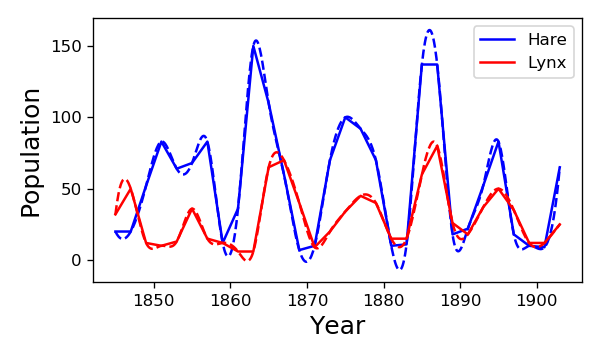
\includegraphics[width=0.97\columnwidth]{images/interpolated.png}
\caption{The original hare and lynx population dataset (in bold), along with the cubic spline interpolation (dotted).}
\label{fig:interpolated}
\end{figure}

\subsection{DMD Results}
We train a DMD model with rank 2 on the first 300 observations, and use the model to predict the population across all the years, following the steps outlined in Section \ref{section:dmd}. As seen in Figure \ref{fig:dmd}, the model performed poorly. Not only do we have a poor fit because of the grossly mismatched period, but we also have negative population predictions, which are biologically implausible.

\begin{figure}[htb] 
\centering
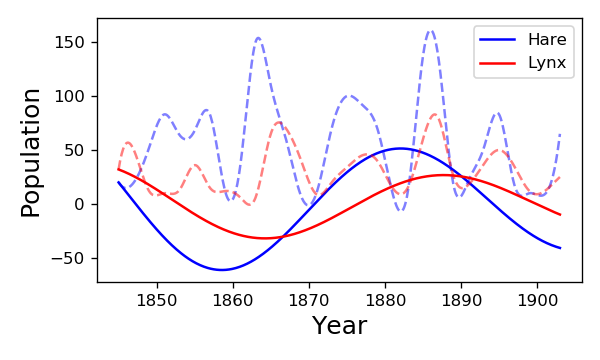
\includegraphics[width=0.97\columnwidth]{images/dmd.png}
\caption{The interpolated dataset (in dots), along with the DMD prediction (in bold).}
\label{fig:dmd}
\end{figure}

However, there are some redeeming qualities of this prediction. First, it manages to produce an oscillatory prediction. When we inspect the DMD eigenvalues, we see that both eigenvalues have real parts that are very close to 1, allowing the predictions to not explode or decay too quickly, with small complex components that allow the predictions to oscillate in time. Second, even with just half the dataset used for training, the model captures the fact that the prey population should rise before the predator population begins to rise.

\subsection{Time-delay Embedding SVD Analysis}
We then apply time-delay embedding to the data, as described in Section \ref{section:time_delay}, to see if the data can be reprojected into a new space where DMD would work better.

We found that using 6 as the embedding degree produced decent results. On applying SVD to the 6-degree time-delay embedded dataset, we found that we need at least 2 modes to capture 99\% of the energy, and 3 modes to capture 99.9\% of the energy, as shown in Figure \ref{fig:time_delayed_energy}. Thus, we believe that there are likely at least 2 latent variables behind the dynamics.

\begin{figure}[htb] 
\centering
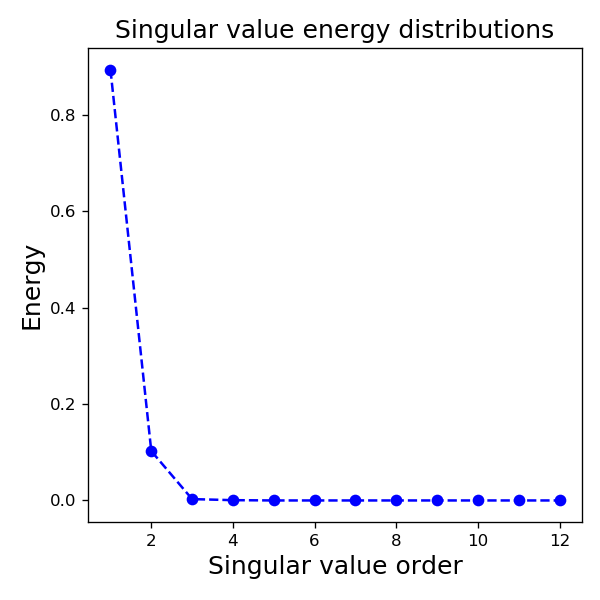
\includegraphics[width=0.97\columnwidth]{images/time_delayed_energy.png}
\caption{Energy distribution of singular values of time-delay embedded data.}
\label{fig:time_delayed_energy}
\end{figure}

The population modes can be seen in Figure \ref{fig:time_delayed_pop_mode}. As discussed in Section \ref{section:svd}, these are obtained from the columns of $V$, which serve as good basis vectors of the rows of the original data. As a reminder, the original rows of the data correspond to the interpolated hare and lynx population time series. The first two modes seem to be phase-offset in nature, with the peaks of the first mode lagging behind the peaks of the second mode. This perhaps captures the phase offset between predator and prey that is also present in the original dataset.

\begin{figure}[htb] 
\centering
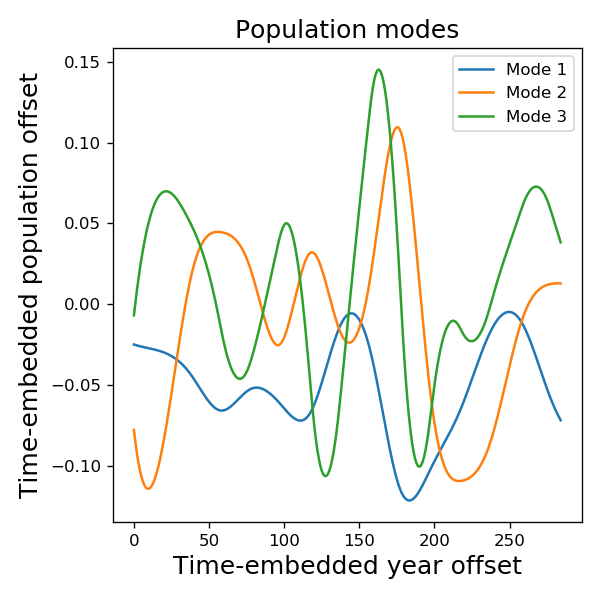
\includegraphics[width=0.97\columnwidth]{images/time_delayed_population_mode.png}
\caption{Population modes of the time-delay embedded data.}
\label{fig:time_delayed_pop_mode}
\end{figure}

The time modes can be seen in Figure \ref{fig:time_delayed_time_mode}. This is harder to interpret because due to time-delay embedding, the hare and lynx populations of each year are interleaved along the columns. The first two modes seem to again be phase-offset. The third mode that seems to increase over time perhaps captures a global increasing or decreasing trend of the interpolated data. 
\begin{figure}[htb] 
\centering
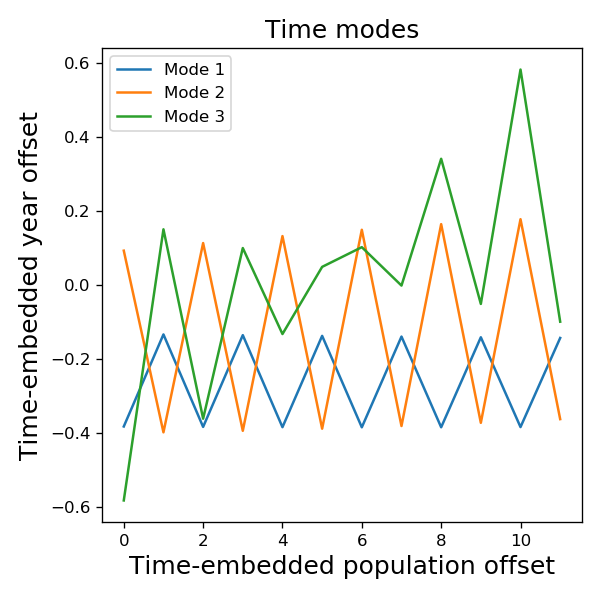
\includegraphics[width=0.97\columnwidth]{images/time_delayed_time_mode.png}
\caption{Time modes of the time-delay embedded data.}
\label{fig:time_delayed_time_mode}
\end{figure}

\subsection{DMD with Time-delay Embedding Results}
From the previous analysis, we decided to stick to 6-degree embedding, and chose 3 for the DMD rank, since the 3 top singular values captures more than 99.9\% of the energy. We then apply DMD on this time-delay embedded dataset. Note that to obtain the predicted hare and lynx population, we extract just the first two rows from the time-delayed embedded matrix.

As seen in Figure \ref{fig:time_delayed_dmd}, the result is much better than the regular DMD, with the prediction obtaining a frequency that is a much better fit to the interpolated data, with the phase offset quality still being retained. Furthermore, this prediction also captures the fact that the hare population has a larger amplitude than that of the lynx. This perhaps indicates that the time-delay embedded space allows the linearity assumptions of DMD to hold better than in the original interpolated data.

\begin{figure}[htb] 
\centering
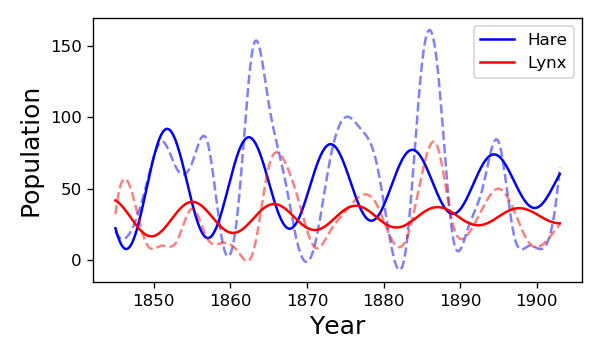
\includegraphics[width=0.97\columnwidth]{images/dmd_time_delay.png}
\caption{The interpolated dataset (in dots), along with the 6-degree time-delay embedded DMD prediction (in bold).}
\label{fig:time_delayed_dmd}
\end{figure}

\subsection{Lotka-Volterra Results}
We obtain the best-fit parameter values for the Lotka-Volterra model, as described in Section \ref{section:lotka_volterra}. As seen in Figure \ref{fig:lotka}, the result seems reasonable. The amplitudes of the predicted hare and lynx populations match those of the interpolated data. Furthermore, the phase offset characteristic where the peaks of hare population precede the peaks of lynx is also captured. The main downside is that the Lotka-Volterra model seems to capture a single peak amplitude, and fails to capture the lower peaks which we see in the original data.

Letting $x$ be the hare population, and $y$ be the lynx population, the recovered equations, up to three decimal places, are as follows.
\begin{equation}
\begin{split}
\frac{dx}{dt} = 0.217 x -0.009 xy \\
\frac{dy}{dt} = -0.381 y + 0.006 xy
\end{split}
\end{equation}

It is interesting to see that the non-linear coefficients are as small as 0.006. This informs us that for our SINDy approaches, we should not carelessly discard small values that capture important non-linear components. In this case, if we had discarded the small non-linear components, we would be left with two exponential solutions without oscillations.

\begin{figure}[htb] 
\centering
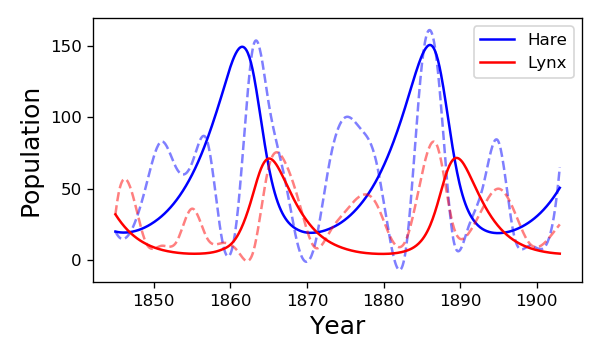
\includegraphics[width=0.97\columnwidth]{images/lotka.png}
\caption{The interpolated dataset (in dots), along with the Lotka-Volterra prediction (in bold).}
\label{fig:lotka}
\end{figure}

\subsection{SINDy Results}
\label{section:sindy_results}
We perform SINDy on the first half of the interpolated dataset to obtain different ODE models, as per Section \ref{section:sindy}. We have tried three different function libraries, corresponding to polynomials of degrees one to three. That is, letting $x$ and $y$ be the hare and lynx population respectively, then the first function library consists of $[x, y]$ and the second function library consists of $[x^2, xy, y^2, x, y]$. For each SINDy run, we obtain the coefficients by running multiple Lasso iterations, with regularization weight $\alpha$ ranging from 0 to 10 in increments of 0.1. We only report the results that give the lowest Frobenius norm of the deviation between the predicted pairs of time series and the interpolated time series for the first half of the dataset. The results can be seen in Table \ref{tbl:sindy_results}.

We discuss the results from function libraries of polynomials of degree 1, 2, and 3, which we will refer to as Poly-1, Poly-2, and Poly-3. The predictions of Poly-3 seems to just be a regression of the mean, with the prediction piercing through the center of the original dataset. The predictions of Poly-2 are very poor, with the hare population going to negative values. Poly-1 seems to be the only model that captures the oscillation in the data, but unfortunately also predicts negative population values. We also note that across all the models, heavier weights are placed onto the lower degree terms, and much smaller weights are placed on the higher degree terms, perhaps due to Lasso discouraging the model from recruiting the complex terms.

Given this discouraging result, we create a final model Poly-3-trimmed by selecting the 4 highest weighted terms from Poly-3: $[x, x^2, xy, y^2]$, and running SINDy on this smaller function library. We were able to see a marked improvement, where the prediction has a weak oscillation, and also stays within the centers of the true timeseries values.
\newcolumntype{M}[1]{>{\centering\arraybackslash}m{#1}}
\newcommand{\addpic}[1]{\includegraphics[width=22em]{#1}}
\newcommand{\addpicr}[1]{\vspace*{-4mm}\includegraphics[width=22em]{#1}}
\begin{table*}[t]
    \centering
    \begin{tabular}{cM{60mm}M{70mm}}
       \toprule
        \midrule
        Poly-1 & \addpic{images/sindy1_pred.png}
        & \addpicr{images/sindy1_coef.png} \\
        Poly-2 & \addpic{images/sindy2_pred.png}
        & \addpicr{images/sindy2_coef.png}  \\
        Poly-3 & \addpic{images/sindy3_pred.png}
        & \addpicr{images/sindy3_coef.png}  \\
        Poly-3-trimmed & \addpic{images/sindy3t_pred.png}
        & \addpicr{images/sindy3t_coef.png}  \\
        \bottomrule
    \end{tabular}
    \caption{SINDy results on library functions with polynomials of degree 1,2 and 3. The last row is the trimmed degree 3 library as described in Section \ref{section:sindy_results}. The left column contains the interpolated dataset (in dots), along with the SINDy predictions (in bold). The right column are the weights assigned to the library functions, as obtained by Lasso with the regularization parameter $\alpha$ stated on the title of each figure.}
    \label{tbl:sindy_results}
\end{table*}

\subsection{KL Divergence Results}
All the previous models have been trained only on the first half of the interpolated data.
We now compare their performances on the unseen second half, by using KL divergence as discussed in Section \ref{section:kl_div}. We will discard DMD, Poly-1 and Poly-2, since they produce negative population predictions, which are biologically implausible.

As seen in Table \ref{tbl:kl_div}, Time-delay embedded DMD seems to perform the best, with the smallest KL divergence of 6.04. Looking at Figure \ref{fig:time_delayed_dmd}, we see that this is the only model that captures the high frequency of the original dataset.

\begin{table}[ht]
\caption{KL Divergence on Test Set (rounded to 2 decimal places)} % title of Table
\centering % used for centering table
\begin{tabular}{c c} 
\hline\hline 
Model & KL Divergence \\
\hline
Time-delay embedded DMD & \textbf{6.04} \\
Lotka-Volterra & 6.21 \\
Poly-3 & 6.28 \\
Poly-3-trimmed & 6.18 \\
\hline %inserts single line
\end{tabular}
\label{tbl:kl_div}
\end{table}

\subsection{AIC and BIC Results}
The drawback from the KL divergence metric is that we are not taking into account model complexity. We also report the AIC and BIC results as described in Section \ref{section:aic_bic}. Note that AIC and BIC is meant to measure the tradeoff between model complexity and data fit on the same dataset, and so we calculate these values solely based on the first half of the dataset. We will also only consider the top 3 models that performed best as measured by KL divergence: Time-delay embedded DMD, Lotka-Volterra and Poly-3-trimmed.

The number of parameters, $k$, for each model, are as follows.
\begin{enumerate}
    \item{Time-delay embedded DMD has 39 parameters in total. This is because the DMD modes $\Phi$ is shaped $n \times r$, which is $12 \times 3$. Note that the 12 comes from the 6-embedding of the hare and lynx population, and 3 is the number of modes we decided to keep. While the DMD modes give us 36 numbers, the 3 DMD eigenvalues bring us to a total of 39.}
    \item{Lotka-Volterra has 4 parameters in total, corresponding to the 2 coefficients for $\frac{dx}{dt}$, and another 2 coefficients for $\frac{dy}{dt}$.}
    \item{Poly-3-trimmed has 8 parameters in total, since we only have 4 library functions, and two state variables.}
\end{enumerate}

\begin{table}[ht]
\caption{AIC and BIC of Top 3 models (rounded to the closest integer)} % title of Table
\centering % used for centering table
\begin{tabular}{c c c} 
\hline\hline 
Model & AIC & BIC \\
\hline
Time-delay embedded DMD & 7282 & 7425 \\
Lotka-Volterra & \textbf{7266} & \textbf{7280} \\
Poly-3-trimmed & 7324 & 7354 \\
\hline %inserts single line
\end{tabular}
\label{tbl:kl_div}
\end{table}

Here we see that the Lotka-Volterra model has the lowest AIC and BIC scores. We now see that even though according to the KL divergence metric, the time-delay embedded DMD was deemed the best model, AIC and BIC metrics successfully take into account the fact that the Lotka-Volterra model has far fewer free parameters to work with, and is hence the better model at balancing data fit and model complexity.

\subsection{Time-delayed Embedded DMD on Chemical Oscillator Movie}
We now move away from the population dataset, and instead focus on the chemical oscillator movie dataset. We focus only on the 40 by 40 square patch as shown in Figure \ref{fig:movie_window}. We will also focus only on the last 50 frames of the video. This setup allows us to focus on the prediction of waves that are propagating diagonally to the bottom right corner.


\begin{figure*}[!t]
\minipage{0.32\textwidth}
  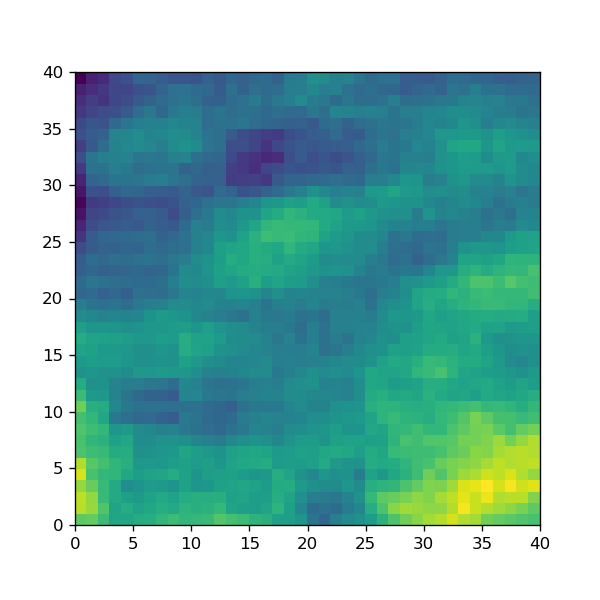
\includegraphics[width=\linewidth]{images/movie_mode1.png}
\endminipage\hfill
\minipage{0.32\textwidth}
  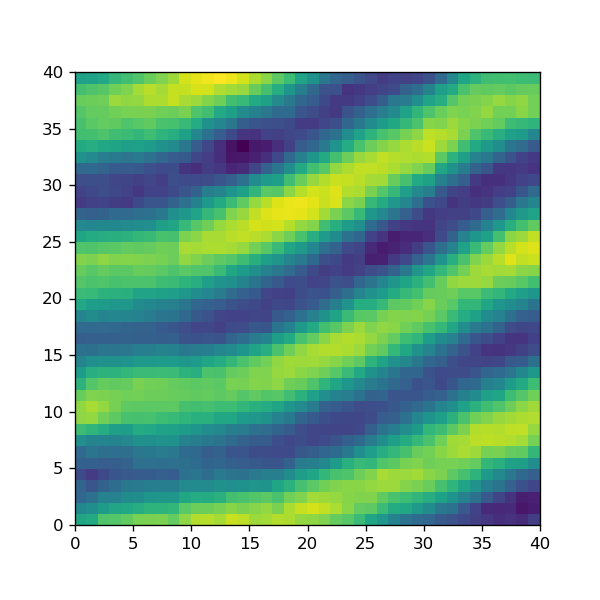
\includegraphics[width=\linewidth]{images/movie_mode2.png}
\endminipage\hfill
\minipage{0.32\textwidth}%
  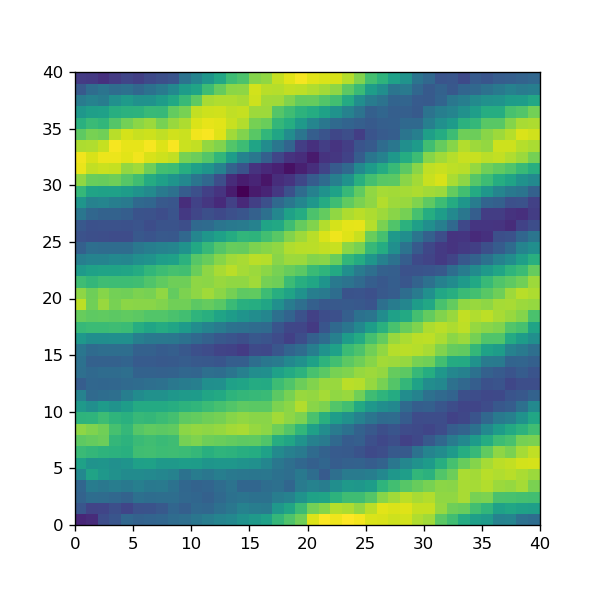
\includegraphics[width=\linewidth]{images/movie_mode3.png}
\endminipage
\caption{The top 3 spatial SVD modes of the training video. On the left is the first mode, on the center is the second mode, and on the right is the third mode.}
\label{fig:movie_mode}
\end{figure*}

\begin{figure*}[!t]
\minipage{0.32\textwidth}
  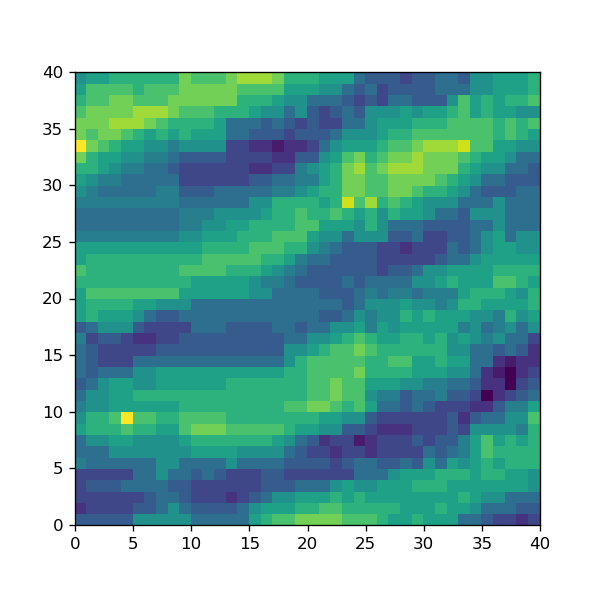
\includegraphics[width=\linewidth]{images/movie_gold.png}
\endminipage\hfill
\minipage{0.32\textwidth}
  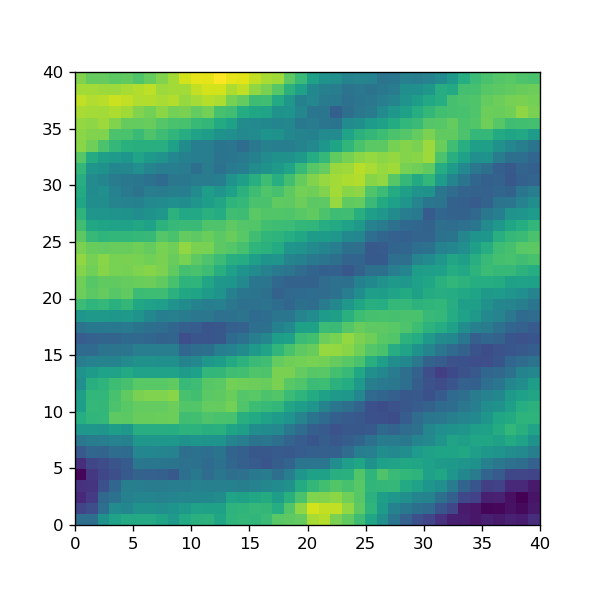
\includegraphics[width=\linewidth]{images/movie_dmd.png}
\endminipage\hfill
\minipage{0.32\textwidth}%
  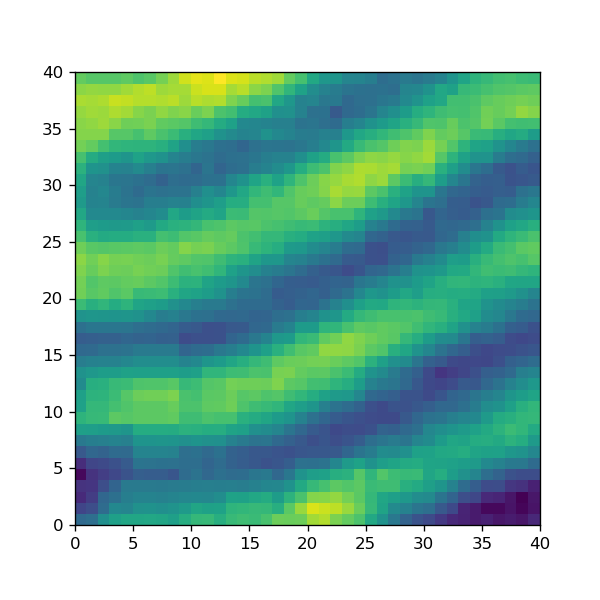
\includegraphics[width=\linewidth]{images/movie_time_delayed_dmd.png}
\endminipage
\caption{On the left is the true 50th frame, on the center is the prediction by DMD, and on the right is the prediction by time-delayed embedded DMD.}
\label{fig:movie_pred}
\end{figure*}

\begin{figure}[htb] 
\centering
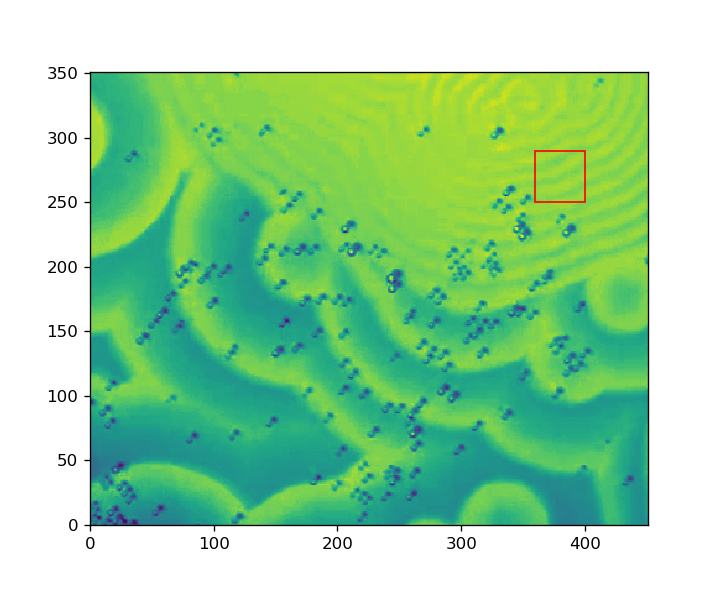
\includegraphics[width=0.97\columnwidth]{images/movie_window.png}
\caption{A frame from the chemical oscillator movie, with the portion to be analyzed outlined by the red square patch.}
\label{fig:movie_window}
\end{figure}

\begin{figure}[htb] 
\centering
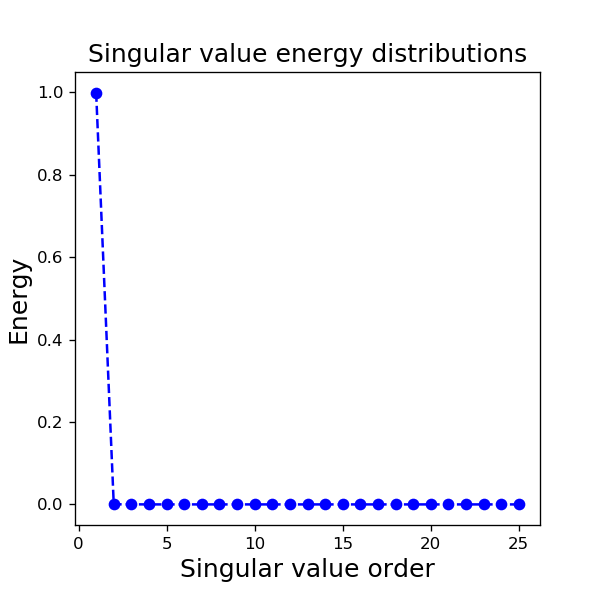
\includegraphics[width=0.97\columnwidth]{images/movie_energy.png}
\caption{Energy distribution of singular values of the training video data.}
\label{fig:movie_energy}
\end{figure}

Our prediction task is to use DMD and time-delay embedded DMD on the first 25 frames, and predict the 50th frame. This is to test if DMD can successfully capture wave propagation in a video data.

We first preprocess the video data into a 2D matrix of size $n \times m$, where $n$ corresponds to the number of pixels and $m$ corresponds to the frame number. We flatten each $40 \times 40$ 2D image into $1600 \times 1$ vectors by taking each transposed image row and concatenating them to form a long column. This gives us the training data matrix of dimension $1600 \times 25$.

We apply SVD to this training data matrix. As seen in Figure \ref{fig:movie_energy}, even the first mode already captures 99.9\% of the energy.

We inspect the first 3 spatial modes (the first 3 column vectors of $U$ from SVD), and de-flatten these vectors into a 2D image. As seen from Figure \ref{fig:movie_mode}, the first mode seems to just capture the static background of the video, whereas the other two modes, which are waves with a phase offset, seems to capture the phenomena of the travelling wave. This was further validated by performing DMD with varying number of modes. With just one or two modes, the predicted video will just be a static image. It is not until we include the third mode that the predicted video starts to result in a propagating wave.

This intuitively makes sense, since DMD tries to reconstruct the predicted frame through a linear combination of these spatial modes. To construct a wave of any phase offset, one would need a linear combination of at least two waves with a non-zero phase offset.

With the above analysis, we apply DMD with rank 3, and time-delayed embedded DMD with rank 3 and embedding degree of 2, onto the first 25 training video frames, and use it to predict the 50th frame.
The results are show on Figure \ref{fig:movie_pred}. We can see that both DMD and time-delayed embedded DMD were able to produce pretty good predictions, although a lot smoother than the actual image. Time-delayed embedded DMD has a slight edge over regular DMD because for the darker patches, it is able to produce darker pixels similar to the original image. 

Overall, this was a very pleasant surprise. DMD is able to reproduce the travelling wave video, even with as little as 3 modes.

%%%%%%%%%%%%%%%%%%%%%%%%%%%%%%%%%%%%%%%%%%%%%%%%%%%%%%%%%%%%%%%%%%%%%%%%%%%%%%%%
\section{Summary and Conclusions}
We have applied various model discovery techniques such as DMD, time-delayed embedding and SINDy on population and video datasets, and compared their performances using evaluation metrics such as KL divergence, AIC and BIC. We showed that these models were able to capture the core dynamics behind the noisy datasets, and were able to make decent predictions of future states that they have not been trained on.

\bibliographystyle{ieeetr}
\bibliography{bibliography}
\clearpage

\onecolumn
%%%%%%%%%%%%%%%%%%%%%%%%%%%%%%%%%%%%%%%%%%%%%%%%%%%%%%%%%%%%%%%%%%%%%%%%%%%%%%%%
\section*{Appendix A: Key Python functions}
\subsection*{Dynamic Mode Decomposition}
\begin{verbatim}
def dmd(data, r):
  """
  Perform dynamic mode decomposition on the data matrix.
  Parameters:
  - data (n x m+1 matrix) Rows are spatial locations and columns are time points.
    That is, there are n spatial locations and m time points.
  - r (int) The low-rank to perform DMD in.
  Returns:
  - Phi (n x r matrix) The DMD (spatial) modes.
  - Lambda (r x r matrix) The diagonal eigenvalue matrix.
  - b (r x 1 matrix). The low-rank initial condition 
  """
  X0 = data[:, :-1]
  X1 = data[:, 1:]

  # X0 is n x m 
  # U is n x n
  # S is n x n, a diagonal matrix of the singular values.
  # Vh is m x m
  U, singular_vals, Vh = np.linalg.svd(X0)
  S = np.diag(singular_vals)
  V = Vh.conj().T
  # Ur is n x r
  Ur = U[:,:r]
  # Sr is r x r
  Sr = S[:r, :r]
  # Vr is m x r
  Vr = V[:,:r]
  Sr_inv = np.linalg.inv(Sr)
  # Atilde is r x r
  Atilde = Ur.conj().T @ X1 @ Vr @ Sr_inv

  # Both W and Lambda are r x r 
  eigenvalues, W = np.linalg.eig(Atilde)
  Lambda = np.diag(eigenvalues)

  # Phi is n x r, the DMD spatial models
  Phi = X1 @ (Vr @ Sr_inv) @ W
  initial_condition = X0[:, 0]
  b = np.linalg.pinv(Phi) @ initial_condition
  
  return Phi, Lambda
\end{verbatim}

\subsection*{Future Prediction from DMD Modes and Eigenvalues}
\begin{verbatim}
def get_xt_from_dmd(num_time, Phi, Lambda, b):
  """
  Predict x_t given the DMD results.
  Parameters:
  - num_time. Number of time points to predict states for.
    We will predict x1, ..., x_num_time, where x1 is the predicted initial condition.
  - Phi, Lambda, b - See dmd()
  Return:
  - A (N x num_time) matrix, where N is the number of spatial coordinates.
    mat[:1] will give you the approximation to x1, the initial condition.
  """
  n = Phi.shape[0]
  r = Phi.shape[1]
  result = np.zeros((n, num_time))
  
  # x(t) = Phi Lambda^{t-1} b
  phi_times_lambda = Phi
  for t in range(num_time):
  	# Sometimes the eigenvalues are complex. We only care about the real part.
    result[:, t] = np.real(phi_times_lambda @ b)
    phi_times_lambda = phi_times_lambda @ Lambda
  return result
\end{verbatim}

\subsection*{Time-delayed Embedding}
\begin{verbatim}
def time_delay_embed(data, k):
  """
  Create a time delay embedding of the data matrix, with k offsets.
  Parameters:
  - data (n x m matrix) Rows are spatial locations and columns are time points.
  - k (int) The number of embeddings to make. k = 1 means no embedding.
  Return:
  - matrix with (k*n rows, m-k+1 columns)
    The first n rows are the first k columns of data ~ data[all_rows, t = 1 -> k]
    The following n rows are the second k columns of data ~ data[all_rows, t = 2 -> k + 1]
    And so on
  """
  n = data.shape[0]
  m = data.shape[1]
  result = np.zeros((n*k, m-k+1))
  for delay_counter in range(k):
    start_row = n * delay_counter
    end_row_exclusive = start_row + n
    start_col = delay_counter
    end_col_exclusive = delay_counter + m-k+1
    result[start_row:end_row_exclusive, :] = data[:, start_col:end_col_exclusive]
  return result
\end{verbatim}

\subsection*{SVD Energy and Mode Plots}
\begin{verbatim}
def plot_energy_from_singular_values(data):
  U, singular_vals, Vh = np.linalg.svd(data)
  squared_singular_vals = np.power(singular_vals, 2)
  energy_values = squared_singular_vals / np.sum(squared_singular_vals)
  fig, ax = plt.subplots(figsize = (5, 5))
  ax.plot(range(1 , len(energy_values) + 1), energy_values, linestyle='--', marker='o', color='b')
  ax.set_xlabel("Singular value order")
  ax.set_ylabel("Energy")
  ax.xaxis.label.set_fontsize(15)
  ax.yaxis.label.set_fontsize(15)
  ax.set_title("Singular value energy distributions", fontdict={'fontsize': 15})
  print("Percent energy covered: %s" % (np.cumsum(energy_values)))
  return fig

def plot_population_modes(data, top_k):
  U, singular_vals, Vh = np.linalg.svd(data)
  fig1, ax = plt.subplots(figsize = (5, 5))
  for k in range(top_k):
    mode = U[:,k]
    ax.plot(range(len(mode)), mode, label = f"Mode {k + 1}")
    ax.set_xlabel("Time-embedded population offset")
    ax.set_ylabel("Time-embedded year offset")
  ax.xaxis.label.set_fontsize(15)
  ax.yaxis.label.set_fontsize(15)
  ax.set_title("Time modes", fontdict={'fontsize': 15})
  ax.legend()

  fig2, ax = plt.subplots(figsize = (5, 5))
  for k in range(top_k):
    mode = Vh[k, :]
    ax.plot(range(len(mode)), mode, label = f"Mode {k + 1}")
    ax.set_xlabel("Time-embedded year offset")
    ax.set_ylabel("Time-embedded population offset")
  ax.xaxis.label.set_fontsize(15)
  ax.yaxis.label.set_fontsize(15)
  ax.set_title("Population modes", fontdict={'fontsize': 15})
  ax.legend()
  return fig1, fig2
\end{verbatim}

\subsection*{Centered Finite Difference}
\begin{verbatim}
def get_dx_dts(xts):
  """
  Use centered finite difference to approximate dx/dt, given x(t)'s
  
  Parameters:
  - xts (n x 1 column vector). The x(t) over time.
  Return:
  - dx_dts ((n-2) x 1 column vector). The time in front and end are removed.
  """
  dt = util.NEW_DT
  dx_dts = np.zeros(len(xts) - 2)
  for i in range(len(dx_dts)):
    dx_dts[i] = (xts[i+2] - xts[i]) / (2.0 * dt)
  return dx_dts
\end{verbatim}

\subsection*{Function Library Matrix for SINDy}
\begin{verbatim}
def gen_library_matrix(measurements, f_lib):
  """
  Generate a matrix of library functions evaluated against the measurements.
  Parameters:
  - measurements (n x m matrix). n is the dimension of each state variable,
    m is the number of timepoints the measurements were taken.
  - f_lib: list((name, fun(x_vec)). A list of 'L' library functions,
    where each function accepts a column from 'measurements' matrix, that is,
    a single state variable vector, snapshotted in time.
  Return:
    m x L matrix, where each column is a single library function evaluated across
    the m measurements.
  """
  n = measurements.shape[0]
  m = measurements.shape[1]
  L = len(f_lib)
  library_mat = np.zeros((m, L))
  
  for i, name_fun in enumerate(f_lib):
    fun = name_fun[1]
    # Apply fun to each column, which represents x(t)
    library_mat[:,i] = np.apply_along_axis(fun, 0, measurements)
  return library_mat
\end{verbatim}

\subsection*{Lotka-Volterra Parameter Fitting}
\begin{verbatim}
def get_best_fit_lotka_volterra_params(data):
  """
  Use linear regression to obtain the parameters for the ODEs below that best fit the data.
  dx/dt = (b-py)x
  dy/dt = (rx-d)y
  
  Parameters:
  - data (n x m matrix) Rows are spatial locations and columns are time points.
  
  Return:
  - b, p, r, d, the ODE parameters.
  """
  # Generate the RHS of Ax = b
  dx_dts = get_dx_dts(data[0,:])
  dy_dts = get_dx_dts(data[1,:])
  
  # Generate the LHS, A of Ax = b
  # Remove the first and last time samples, because finite difference removes them too.
  data_without_ends = data[:, 1:-1]
  # For dx/dt, our library is [x, -xy]
  # The shape is 28 (time) x 2 (number of library functions)
  x_library = gen_library_matrix(data_without_ends, [
    ("x", lambda x: x[0]),
    ("-xy", lambda x: -x[0] * x[1])
  ])
  # For dy/dt, our library is [-y, xy]
  y_library = gen_library_matrix(data_without_ends, [
    ("-y", lambda x: -x[1]),
    ("xy", lambda x: x[0] * x[1])
  ])
  model = linear_model.LinearRegression()
  
  model.fit(x_library, dx_dts)
  x_library_coefs = model.coef_
  b = x_library_coefs[0]
  p = x_library_coefs[1]
  model.fit(y_library, dy_dts)
  y_library_coefs = model.coef_
  d = y_library_coefs[0]
  r = y_library_coefs[1]
  return b, p, r, d
\end{verbatim}

\subsection*{SINDy Coefficient Finding}
\begin{verbatim}
def get_sindy_params(data, regression_model, f_lib):
  """
  Use sparse regression to obtain the parameters for the ODEs below that best fit the data.
  dx/dt, and dy/dt are linear combinations of (x, y, x2, xy, y, x3, x2y, xy2, y3)
  Note that there are 9 terms.
  That is, we are doing SINDy, but with library functions of polynomials up to degree 3.
  
  Parameters:
  - data (n x m matrix) Rows are spatial locations and columns are time points.
  - regression_model. A scipy regression model to solve Ax = b
  Return:
  - an array of 9 numbers, which are the weights for (x, y, x2, xy, y2, x3, x2y, xy2, y3)
  """
  # Generate the RHS of Ax = b
  dx_dts = get_dx_dts(data[0,:])
  dy_dts = get_dx_dts(data[1,:])
  
  # Generate the LHS, A of Ax = b
  # Remove the first and last time samples, because finite difference removes them too.
  data_without_ends = data[:, 1:-1]
  # The shape is 28 (time) x 2 (number of library functions)
  x_library = gen_library_matrix(data_without_ends, f_lib)
  y_library = gen_library_matrix(data_without_ends, f_lib)
  
  regression_model.fit(x_library, dx_dts)
  dx_library_coefs = regression_model.coef_

  regression_model.fit(y_library, dy_dts)
  dy_library_coefs = regression_model.coef_
  return dx_library_coefs, dy_library_coefs
\end{verbatim}

\subsection*{SINDy Prediction by Solving ODE}
\begin{verbatim}
def generate_predictions_from_sindy(x_library_coefs, y_library_coefs, f_lib):
  """
  Generate the predicted population formatted as the original data
  by using ODE generated by SINDy. Please see get_sindy_params.
  That is, from 1845 to 1903 in increment of 2 years, a 2 x 30 matrix
  Parameters:
  - poly_weights. The return value of get_sindy_params.
  Return:
  - scipy's integrate sol obj. sol.y gives you the predictions.
    sol.success tells you if the integration was successful.
  """
  def dyn(t, states):
    dx = 0
    dy = 0
    for i, name_f in enumerate(f_lib):
      f = name_f[1]
      f_res = f(states)
      dx += x_library_coefs[i] * f_res
      dy += y_library_coefs[i] * f_res
    return np.array([dx, dy])

  # 1845 to 1903 spans 58 years. Each unit time is 1 year. Let t = 0 be year 1845.
  t_max = 58
  t_span = [0, t_max]
  t_eval = np.arange(0, t_max + util.NEW_DT, util.NEW_DT)
  # Hare and lynx population in 1845
  init_conds = [20, 32]
  sol = integrate.solve_ivp(dyn, t_span, init_conds, method = 'RK45', t_eval = t_eval)
  return sol
\end{verbatim}

\subsection*{Joint Probability Distribution Extraction from Population Data}
\begin{verbatim}
def get_population_joint_distribution(population_data, pseudocount = 0.001):
  """
  Parameters
  - data (2 x m matrix) Rows are population types and columns are time points.
  - pseudocount. Laplacian smoothing parameter for never-seen samples.
  Returns
  - 200 x 200 float matrix where mat[i, j] is P(hare = i, lynx = j) at any time point.
    The joint probability is guaranteed to add up to 1 when summed over the entire sample space.
  """
  counts = np.zeros((200, 200))
  # Additive smoothing. For unseen, assume a pseudocount.
  counts += pseudocount
  for t in range(population_data.shape[1]):
    hare = int(population_data[0, t])
    lynx = int(population_data[1, t])
    counts[hare, lynx] += 1
  counts /= np.sum(counts)
  return counts
\end{verbatim}

\subsection*{KL Divergence}
\begin{verbatim}
def get_kl_divergence(gold_distribution, pred_distribution):
  """
  Compute KL divergence of two probability distributions produced by
  get_population_joint_distribution()
  The sample space is all possible integer (hare, lynx) pairs from 0 to 200.
  """
  result = 0
  for hare in range(gold_distribution.shape[0]):
    for lynx in range(gold_distribution.shape[1]):
      p = gold_distribution[hare, lynx]
      q = pred_distribution[hare, lynx]
      result += p * np.log(p/q)
  return result
\end{verbatim}


\subsection*{AIC and BIC}
\begin{verbatim}
def get_aic_bic(k, population_data, predictions):
  """
  Compute AIC and BIC for the provided gold population data and the given
  set of predictions.
  For the likelihood, we assume that each sample in time (a hare and lynx population)
  is independently from a time-invariant joint probability distribution interpolated from
  predictions.
  Parameters
  - k. The number of optimizable free parameters of the model.
  - population_data (2 x m matrix) Rows are population types and columns are time points.
    This is the gold standard
  - predictions (2 x m matrix) The predictions
  """
  n = population_data.shape[1]
  pred_distribution = get_population_joint_distribution(predictions)
  ll_tot = 0
  # Log likelihood of entire datast is the sum of log likelihood of each time step,
  # assumed to be independent
  for t in range(n):
    hare = int(population_data[0,t])
    lynx = int(population_data[1,t])
    # This is the probability of observing this one time point.
    p = pred_distribution[hare, lynx]
    ll_tot += np.log(p)
  
  aic = 2 * k - 2 * ll_tot
  bic = np.log(n) * k - 2 * ll_tot
  return aic, bic
\end{verbatim}

%%%%%%%%%%%%%%%%%%%%%%%%%%%%%%%%%%%%%%%%%%%%%%%%%%%%%%%%%%%%%%%%%%%%%%%%%%%%%%%%
\section*{Appendix B: Supporting Python codes}
The rest of the supporting Python codes can be found on \url{https://github.com/sjonany/AMATH563-public/tree/master/hw2/code}
\end{document}